\section{Example of a LaTeX document}

\subsection{Introduction}

\begin{definition}{Definition Title}\\
    This is a definition.
    \begin{itemize}
        \item This is an itemized list
        \item Should provide a concise explanation
    \end{itemize}
\end{definition}

\begin{concept}{Concept Title}\\
    This is a concept. This describes more general concepts and ideas.
\end{concept}

\begin{lemma}{Lemma Title}\\
    This is a lemma.
\end{lemma}

\begin{theorem}{Theorem Title}\\
    This is a theorem. Also use this for certain explanations that are more on the mathematical side, even if they are not theorems.
\end{theorem}

\begin{corollary}{Corollary Title}\\
    This is a corollary. Also use this for certain explanations that are more on the mathematical side, even if they are not corollaries. 
    Especially in context to a theorem block above, this adds further information or explanations.
    \begin{enumerate}
        \item This is an enumerated item.
        \item This is another enumerated item.
    \end{enumerate}
\end{corollary}

\begin{example}
    this is a simple example. no title required.
\end{example}

\begin{example2}{Example Title}\\
    this is a more complex example. title required.
\end{example2}

\begin{example2}{Example Title}\\
    One can achieve better readability by seperating the task definition (exercise)
    \tcblower
    from the solution (solution).
\end{example2}

\subsubsection{Code and Formulas}

\begin{code}{Code Title}\\
    This is a code block, where general concepts are explained.
\begin{lstlisting}[language=Java, style=basesmol]
// Indentation matters in these blocks, so all the way to the left!
def exampleFunction(param1, param2):
    // This is a comment
    return param1 + param2
\end{lstlisting}

    Depending on the programming language, we need to specify the language for the code block. Style should always be set to style=basesmol.

\begin{lstlisting}[language=C, style=basesmol]
// Indentation matters in these blocks, so all the way to the left!
int example_function(int param1, int param2) {
    // This is a comment
    return param1 + param2;
}
\end{lstlisting}

    \important{Important note:} Within lstlisting blocks we should only include ENGLISH comments. 
    Within the lstlisting environment letters like ä, ö, ü, ß are not supported.
\end{code}

\begin{examplecode}{Example Code Title}\\
    This is an example code block. This should show specific implementations or examples.
\begin{lstlisting}[language=Python, style=basesmol]
# Indentation matters in these blocks, so all the way to the left!
def example_function(param1, param2):
    # This is a comment
    return param1 + param2
\end{lstlisting}
\end{examplecode}

\begin{formula}{Formula Title}\\
This is a formula. This should be used for very important formulas and concepts that can be simplified into a step-by-step process.

    Short formula:
    $E = mc^2$

    Complex formula:
    $$
    \int_{a}^{b} f(x) \, dx = F(b) - F(a)
    $$

    do not use the \texttt{equation} environment, as I prefer working with \$ and \$\$ for inline and block formulas.
\end{formula}

\begin{KR}{KR Title}\\
    This is a KR. This "Kochrezept" is a recipe for a specific exercise type. It should be used for very important recipes and concepts.
    \paragraph{First step}
    This is the first step of the recipe.
    \begin{itemize}
        \item Paragraphs are used to achieve coarse-grained separation of the steps.
        \item Lists within the paragraphs are used to achieve fine-grained separation of the steps.
    \end{itemize}
    \paragraph{Second step}
    and so on.
    \paragraph{conclusion}
    This is the conclusion of the recipe. It should summarize the steps and provide a final overview of the process.
\end{KR} 

\subsection{Special Cases}

\begin{definition}{Definition Title}
    \begin{itemize}
        \item this is an itemized list
    \end{itemize}
    if after a title there is a list, no need to add a new line manually.
\end{definition}

\begin{definition}{Definition Title}
    \\
    %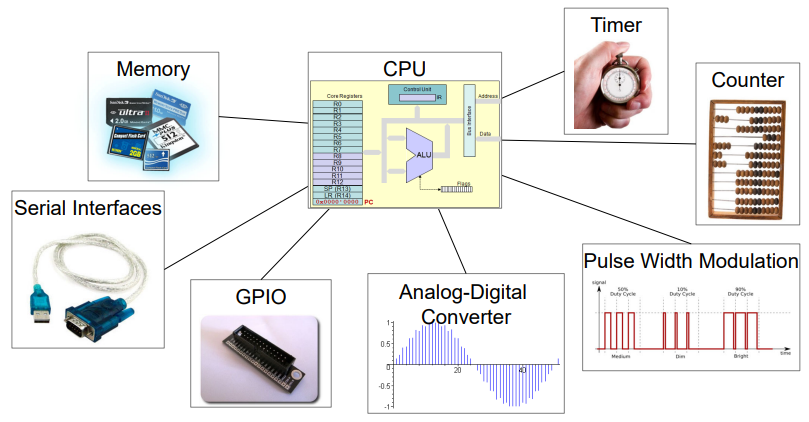
\includegraphics[width=\linewidth]{single_chip_solution.png}
    \\
    before and after an image, we need to add a new line manually. 
\end{definition}

\begin{remark}
    Some characters are treated as special characters in LaTeX. For example, the dollar sign (\$) is used to indicate math mode, and the backslash (\textbackslash) is used to escape special characters. 
    To include these characters in your text, you need to use a backslash before them. 
    For example, to include a dollar sign in your text, you would write \$.
    More examples:
    \begin{itemize}
        \item \&
        \item \%
        \item \{\}
        \item \_
        \item \textbackslash
        \item \textasciitilde
        \item \textasciicircum
    \end{itemize}
\end{remark}

\begin{remark}
    Some characters even need to be defined within a math environment. This can be done inline to show things like $\theta$ or $\alpha$.
    Examples:
    \begin{itemize}
        \item $\neq$
        \item $\sim$
        \item $\approx$
        \item $\leq$
        \item $\geq$
        \item $\in$
        \item $\forall$
        \item $\exists$
        \item $\nexists$
        \item $\subseteq$
        \item $\subsetneq$
        \item $\infty$
    \end{itemize}

    We also use $\rightarrow$ and $\Rightarrow$ for arrows. The first one is a single arrow, the second one is a double arrow.
    These are nice to use in all kinds of contexts, especially when we want to show a transition from one state to another, or some kind of conclusion or extra information.
\end{remark}

\begin{formula}{Formula Title}\\
    In formulas, we have LateX functions that are used to create nice looking formulas.
    examples:
    \begin{itemize}
        \item \texttt{frac} for fractions: $\frac{a}{b}$
        \item \texttt{sqrt} for square roots: $\sqrt{a}$
        \item \texttt{sqrt[n]} for n-th roots: $\sqrt[n]{a}$
        \item \texttt{abs} for absolute values: $|a|$
        \item \texttt{sum} for summation: $\sum_{i=1}^{n} i$
        \item \texttt{prod} for product: $\prod_{i=1}^{n} i$
        \item \texttt{int} for integrals: $\int_{a}^{b} f(x) \, dx$
        \item \texttt{lim} for limits: $\lim_{x \to \infty} f(x)$
        \item \texttt{log} for logarithms: $\log_{b}(a)$
        \item \texttt{ln} for natural logarithms: $\ln(a)$
        \item \texttt{exp} for exponentials: $e^{x}$
        \item \texttt{overline} for overlines: $\overline{a}$
        \item \texttt{underline} for underlines: $\underline{a}$
        \item \texttt{vec} for vectors: $\vec{a}$
        \item \texttt{hat} for hats: $\hat{a}$
        \item \texttt{underbrace} for underbraces: $\underbrace{a}_{b}$
        \item \texttt{overbrace} for overbraces: $\overbrace{a}^{b}$
    \end{itemize}

    If we want to display vectors or matrices, we can use the \texttt{pmatrix} environment. This is a nice way to display matrices in a clean and readable way.

    This is a matrix with m rows and n columns. The \texttt{pmatrix} environment is used to create a matrix with parentheses around it. We can also use the \texttt{bmatrix} environment for square brackets, or the \texttt{vmatrix} environment for vertical bars.
    
    Personally, I prefer using \texttt{psmallmatrix, bsmallmatrix, vsmallmatrix} for my summaries. This is a nice way to display matrices in a clean and readable way.
    
    Generally I use psmallmatrix for vectors, and bsmallmatrix for matrices. vsmallmatrix is usually used in a context where I want to display multiple matrices next to each other (like when showing how the Gauss algorithm works).

    $\begin{psmallmatrix} 1 & 2 & 3 \end{psmallmatrix}$ and $\begin{psmallmatrix} 1 \\ 2 \\ 3 \end{psmallmatrix}$ are both vectors, but the first one is a row vector and the second one is a column vector.
    $$\begin{bsmallmatrix} 1 & 2 & 3 \\ 4 & 5 & 6 \end{bsmallmatrix}$$ is a matrix with 2 rows and 3 columns.
    $$\begin{vsmallmatrix} 1 & 2 & 3 \\ 4 & 5 & 6 \end{vsmallmatrix}$$ is a matrix with 2 rows and 3 columns, but it is displayed in a different way.
\end{formula}




        

    




